\documentclass[../AnalisiDeiRequisiti.tex]{subfiles}


\begin{document}
\section{Casi d'uso}
	\hypertarget{UCG}{}
\subsection{Caso d'uso UCG: Utilizzo generale del prototipo}

        \begin{figure}[!h]
            \centering
            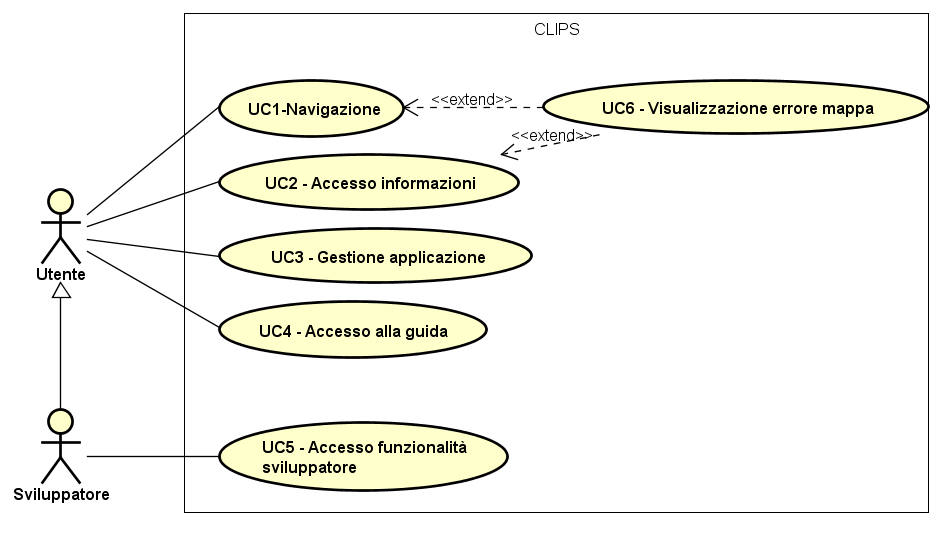
\includegraphics[scale=0.95, width=\textwidth]{img/UCG.png}
            \caption{Caso d'uso UCG: Utilizzo generale del prototipo}\label{fig:UCG} 
        \end{figure}
\begin{itemize}
\item \textbf{Attori}: utente, sviluppatore;
\item \textbf{Descrizione}: un utente deve poter accedere alla navigazione, consultare informazioni relative all'edificio nel suo complesso o a singole aree, modificare le impostazioni utente ed accedere alla guida dell'applicazione. Uno sviluppatore, oltre ad ereditare tutti i casi d'uso di utente, deve poter accedere alle funzionalità avanzate dell'applicazione; 
      \item \textbf{Precondizione}: l'utente ha avviato l'applicazione installata nel proprio dispositivo;

        \item \textbf{Flusso principale degli eventi}:
          \begin{enumerate}
          \item L'utente può accedere alla navigazione (\hyperlink{UC1}{UC1});
          \item L'utente può accedere alle informazioni relative all'intero edificio o a singole aree dell'edificio (\hyperlink{UC2}{UC2});
          \item L'utente può accedere alla gestione dell'applicazione (\hyperlink{UC3}{UC3});
          \item L'utente può accedere alla guida (\hyperlink{UC4}{UC4});
          \item Lo sviluppatore può accedere alle funzionalità avanzate (\hyperlink{UC5}{UC5});

      \end{enumerate}
    \item \textbf{Scenari Alternativi}:
      \begin{enumerate}
          \item Nel caso in cui l'utente voglia accedere alla navigazione di un edificio la cui mappa non risulti aggiornata o presente nel dispositivo viene presentato un errore (\hyperlink{UC6}{UC6});
          \item Nel caso in cui l'utente voglia accedere alle informazioni di un edificio la cui mappa non risulti aggiornata o presente nel dispositivo viene presentato un errore (\hyperlink{UC6}{UC6});

      \end{enumerate}
    \item \textbf{Postcondizione}: il sistema ha erogato le funzionalità richieste dall'utente.
  \end{itemize}
\hypertarget{UC1}{}
\subsection{Caso d'uso UC1: Navigazione}

        \begin{figure}[!h]
            \centering
            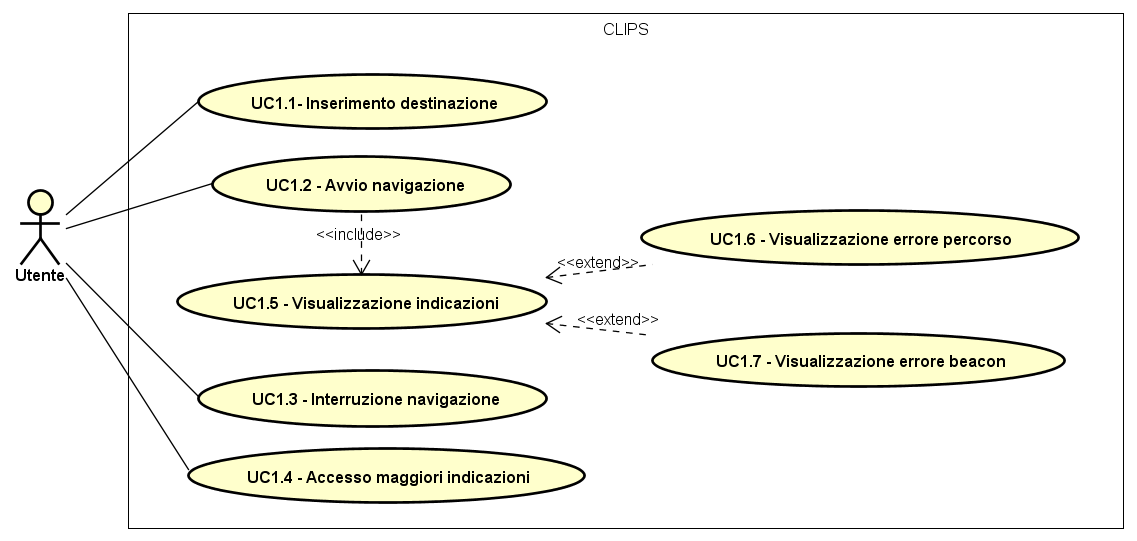
\includegraphics[scale=0.95, width=\textwidth]{img/UC1.png}
            \caption{Caso d'uso UC1: Navigazione}\label{fig:UC1} 
        \end{figure}
\begin{itemize}
\item \textbf{Attori}: utente;
\item \textbf{Descrizione}: l'utente deve poter essere guidato dal sistema verso una destinazione scelta. Quando l'utente si trova in navigazione deve poter: interrompere la navigazione in corso, accedere ad indicazioni più dettagliate; 
      \item \textbf{Precondizione}: l'utente si trova nella sezione dedicata alla navigazione, ha attivato il Bluetooth, si trova all'interno di un edificio mappato, il dispositivo deve rilevare almeno un beacon
;

        \item \textbf{Flusso principale degli eventi}:
          \begin{enumerate}
          \item L'utente indica la destinazione che vuole raggiungere (\hyperlink{UC1.1}{UC1.1});
          \item L'utente avvia la navigazione verso la destinazione scelta (\hyperlink{UC1.2}{UC1.2});
          \item L'utente può interrompere la navigazione in corso  (\hyperlink{UC1.3}{UC1.3});
          \item L'utente può accedere ad indicazioni più dettagliate  (\hyperlink{UC1.4}{UC1.4});

      \end{enumerate}
    \item \textbf{Estensioni}:
      \begin{enumerate}
          \item Visualizzazione errore mappa (\hyperlink{UC6}{UC6});

      \end{enumerate}
    \item \textbf{Scenari Alternativi}:
      \begin{enumerate}
          \item Nel caso in cui l'utente non rispetti le indicazioni relative al percorso proposto viene visualizzato un errore (\hyperlink{UC1.6}{UC1.6});
          \item Nel caso in cui l'utente si trovi in un luogo non coperto dal segnale di almeno un beacon viene visualizzato un errore (\hyperlink{UC1.7}{UC1.7});

      \end{enumerate}
    \item \textbf{Postcondizione}: l'utente ha raggiunto la destinazione scelta oppure ha interrotto la navigazione.
  \end{itemize}
\hypertarget{UC1.1}{}
\subsection{Caso d'uso UC1.1: Inserimento destinazione}

        \begin{figure}[!h]
            \centering
            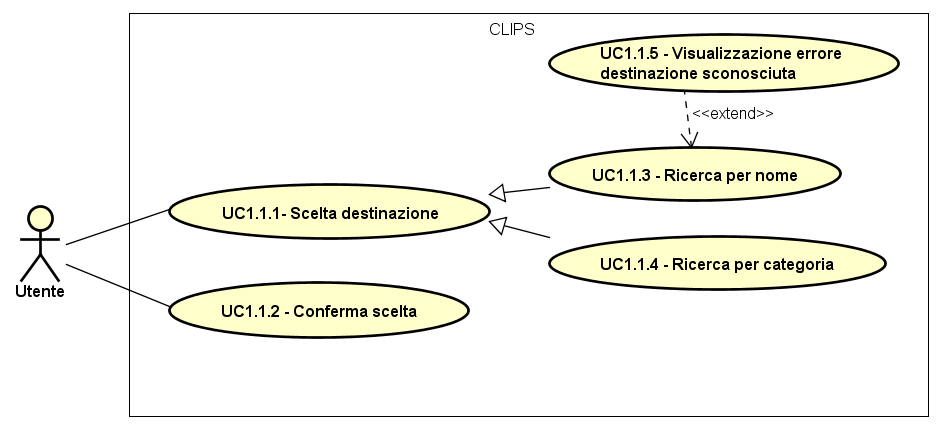
\includegraphics[scale=0.95, width=\textwidth]{img/UC1-1.png}
            \caption{Caso d'uso UC1.1: Inserimento destinazione}\label{fig:UC1.1} 
        \end{figure}
\begin{itemize}
\item \textbf{Attori}: utente;
\item \textbf{Descrizione}: l'utente deve poter scegliere ed inserire una destinazione da raggiungere, tra le destinazioni previste; 
      \item \textbf{Precondizione}: l'utente si trova nella sezione dedicata alla scelta della destinazione e il dispositivo rileva la presenza di un beacon;

        \item \textbf{Flusso principale degli eventi}:
          \begin{enumerate}
          \item L'utente sceglie una destinazione  (\hyperlink{UC1.1.1}{UC1.1.1});
          \item L'utente conferma la destinazione scelta  (\hyperlink{UC1.1.2}{UC1.1.2});

      \end{enumerate}
    \item \textbf{Scenari Alternativi}:
      \begin{enumerate}
          \item Nel caso in cui l'utente ricerchi per nome una destinazione non prevista viene visualizzato un errore (\hyperlink{UC1.1.5}{UC1.1.5});

      \end{enumerate}
    \item \textbf{Postcondizione}: la destinazione da raggiungere è stata impostata.
  \end{itemize}
\hypertarget{UC1.1.1}{}
\subsection{Caso d'uso UC1.1.1: Scelta destinazione}
\begin{itemize}
\item \textbf{Attori}: utente;

        \item \textbf{Generalizzazione di:}:
          \begin{enumerate}
          \item Ricerca per nome (\hyperlink{UC1.1.3}{UC1.1.3});
          \item Ricerca per categoria (\hyperlink{UC1.1.4}{UC1.1.4});

      \end{enumerate}
\item \textbf{Descrizione}: l'utente deve poter scegliere una destinazione interna all'edificio, tra quelle conosciute dal sistema; 
      \item \textbf{Precondizione}: l'utente si trova nella sezione dedicata all'inserimento della destinazione;
    \item \textbf{Postcondizione}: la destinazione è stata scelta.
  \end{itemize}
\hypertarget{UC1.1.2}{}
\subsection{Caso d'uso UC1.1.2: Conferma scelta}
\begin{itemize}
\item \textbf{Attori}: utente;
\item \textbf{Descrizione}: l'utente si trova nella sezione dedicata alla conferma della destinazione; 
      \item \textbf{Precondizione}: l'utente ha selezionato una destinazione prevista;
    \item \textbf{Postcondizione}: la destinazione scelta è stata confermata.
  \end{itemize}
\hypertarget{UC1.1.3}{}
\subsection{Caso d'uso UC1.1.3: Ricerca per nome}
\begin{itemize}
\item \textbf{Attori}: utente;
\item \textbf{Descrizione}: l'utente deve poter inserire il nome di una destinazione che vuole raggiungere; 
      \item \textbf{Precondizione}: l'utente si trova nella sezione dedicata alla ricerca per nome della destinazione;
    \item \textbf{Estensioni}:
      \begin{enumerate}
          \item Visualizzazione errore destinazione sconosciuta (\hyperlink{UC1.1.5}{UC1.1.5});

      \end{enumerate}
    \item \textbf{Postcondizione}: l'utente ha scelto la destinazione desiderata.
  \end{itemize}
\hypertarget{UC1.1.4}{}
\subsection{Caso d'uso UC1.1.4: Ricerca per categoria}
\begin{itemize}
\item \textbf{Attori}: utente;
\item \textbf{Descrizione}: l'utente deve poter cercare la destinazione che vuole raggiungere ricercandola tra le categorie proposte dal sistema rispettivamente all'edificio nel quale si trova l'utente; 
      \item \textbf{Precondizione}: l'utente si trova nella sezione dedicata alla ricerca per categoria della destinazione;
    \item \textbf{Postcondizione}: l'utente ha scelto la destinazione desiderata.
  \end{itemize}
\hypertarget{UC1.1.5}{}
\subsection{Caso d'uso UC1.1.5: Visualizzazione errore destinazione sconosciuta}
\begin{itemize}
\item \textbf{Descrizione}: l'utente ha indicato una destinazione sconosciuta al sistema; 
      \item \textbf{Precondizione}: l'utente ha effettuato la ricerca della destinazione per nome ed ha confermato la scelta di una destinazione;
    \item \textbf{Postcondizione}: viene notificato all'utente che la destinazione indicata è sconosciuta al sistema.
  \end{itemize}
\hypertarget{UC1.2}{}
\subsection{Caso d'uso UC1.2: Avvio navigazione}
\begin{itemize}
\item \textbf{Attori}: utente;
\item \textbf{Descrizione}: l'utente deve poter avviare la navigazione in modo che il sistema calcoli il percorso e le relative indicazioni per guidare l'utente verso la destinazione scelta. Le indicazioni sono fornite in forma testuale; 
      \item \textbf{Precondizione}: l'utente ha inserito una destinazione valida e il dispositivo rileva la presenza di un beacon;
    \item \textbf{Inclusioni}:
      \begin{enumerate}
          \item Visualizzazione indicazioni (\hyperlink{UC1.5}{UC1.5});

      \end{enumerate}
    \item \textbf{Postcondizione}: il sistema ha fornito le indicazioni basilari  e necessarie all'utente per muoversi dalla sua posizione attuale alla destinazione scelta, rispettando le preferenze indicate dall'utente.
  \end{itemize}
\hypertarget{UC1.3}{}
\subsection{Caso d'uso UC1.3: Interruzione navigazione}
\begin{itemize}
\item \textbf{Attori}: utente;
\item \textbf{Descrizione}: l'utente deve poter interrompere la navigazione in corso; 
      \item \textbf{Precondizione}: l'utente ha avviato la navigazione;
    \item \textbf{Postcondizione}: la navigazione è stata interrotta e l'utente è stato riportato alla schermata principale dell'applicazione.
  \end{itemize}
\hypertarget{UC1.4}{}
\subsection{Caso d'uso UC1.4: Accesso a maggiori indicazioni}

        \begin{figure}[!h]
            \centering
            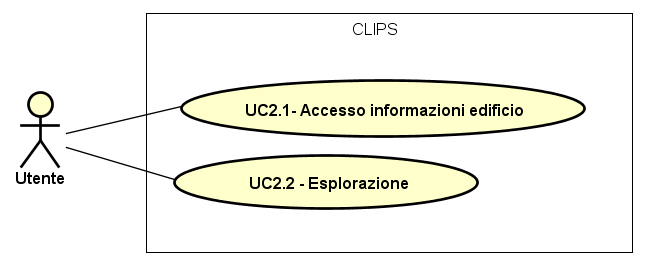
\includegraphics[scale=0.95, width=\textwidth]{img/UC1-4.png}
            \caption{Caso d'uso UC1.4: Accesso a maggiori indicazioni}\label{fig:UC1.4} 
        \end{figure}
\begin{itemize}
\item \textbf{Attori}: utente;
\item \textbf{Descrizione}: l'utente deve poter accedere ad indicazioni dettagliate che lo possano aiutare durante la navigazione; 
      \item \textbf{Precondizione}: l'utente ha avviato la navigazione e si trova nella sezione dedicata a fornire le informazioni più dettagliate;

        \item \textbf{Flusso principale degli eventi}:
          \begin{enumerate}
          \item L'utente può accede alle foto della prossima area (\hyperlink{UC1.4.1}{UC1.4.1});
          \item L'utente può accedere alle indicazioni testuali estese (\hyperlink{UC1.4.2}{UC1.4.2});
          \item L'utente può accedere alla lista delle indicazioni utili per raggiungere, dall'area in cui si trova, la destinazione scelta (\hyperlink{UC1.4.3}{UC1.4.3});

      \end{enumerate}
    \item \textbf{Postcondizione}: il sistema ha presentato all'utente informazioni dettagliate in supporto alla navigazione corrente.
  \end{itemize}
\hypertarget{UC1.4.1}{}
\subsection{Caso d'uso UC1.4.1: Accesso foto della prossima area}
\begin{itemize}
\item \textbf{Attori}: utente;
\item \textbf{Descrizione}: l'utente deve poter accedere alle foto che ritraggono la prossima area prevista dal percorso, in modo da poterla individuare più facilmente; 
      \item \textbf{Precondizione}: le foto relative alla prossima area esistono e devono poter essere recuperate dall'applicazione;
    \item \textbf{Postcondizione}: il sistema ha presentato all'utente delle foto relative alla prossima area.
  \end{itemize}
\hypertarget{UC1.4.2}{}
\subsection{Caso d'uso UC1.4.2: Accesso indicazione testuale estesa}
\begin{itemize}
\item \textbf{Attori}: utente;
\item \textbf{Descrizione}: l'utente deve poter accedere ad indicazioni più dettagliate che possano aiutarlo a raggiungere la prossima area; 
      \item \textbf{Precondizione}: le indicazioni dettagliate relative alla prossima area esistono e devono poter essere recuperate dall'applicazione;
    \item \textbf{Postcondizione}: il sistema ha presentato all'utente indicazioni testuali dettagliate per raggiungere la prossima area.
  \end{itemize}
\hypertarget{UC1.4.3}{}
\subsection{Caso d'uso UC1.4.3: Accesso lista indicazioni}
\begin{itemize}
\item \textbf{Attori}: utente;
\item \textbf{Descrizione}: l'utente deve poter accedere alla lista completa delle indicazioni da seguire, a partire dall'area in cui si trova, per raggiungere la destinazione scelta; 
      \item \textbf{Precondizione}: la lista che riporta tutte le indicazioni da seguire per raggiungere la destinazione, a partire dall'area in cui si trova l'utente, deve essere disponibile;
    \item \textbf{Postcondizione}: il sistema ha presentato all'utente la lista delle indicazioni richieste.
  \end{itemize}
\hypertarget{UC1.5}{}
\subsection{Caso d'uso UC1.5: Visualizzazione indicazioni}
\begin{itemize}

\item \textbf{Descrizione}: il sistema presenta all'utente le indicazioni utili alla navigazione; 
      \item \textbf{Precondizione}: l'utente ha avviato la navigazione;
    \item \textbf{Estensioni}:
      \begin{enumerate}
          \item Visualizzazione errore percorso (\hyperlink{UC1.6}{UC1.6});
          \item Visualizzazione errore beacon (\hyperlink{UC1.7}{UC1.7});

      \end{enumerate}
    \item \textbf{Postcondizione}: il sistema ha presentato all'utente le indicazioni per raggiungere la destinazione scelta.
  \end{itemize}
\hypertarget{UC1.6}{}
\subsection{Caso d'uso UC1.6: Visualizzazione errore percorso}
\begin{itemize}
    \item \textbf{Precondizione}: i beacon rilevati dal sistema non corrispondono a quelli previsti dal percorso calcolato;
    \item \textbf{Postcondizione}: il sistema ha presentato all'utente un errore relativo al percorso errato.
  \end{itemize}
\hypertarget{UC1.7}{}
\subsection{Caso d'uso UC1.7: Visualizzazione errore beacon}
\begin{itemize}
    \item \textbf{Precondizione}: il dispositivo non è in grado di rilevare alcun beacon;
    \item \textbf{Postcondizione}: il sistema ha presentato all'utente un errore relativo all'impossibilità di rilevare beacon.
  \end{itemize}
\hypertarget{UC2}{}
\subsection{Caso d'uso UC2: Accesso alle informazioni}

        \begin{figure}[!h]
            \centering
            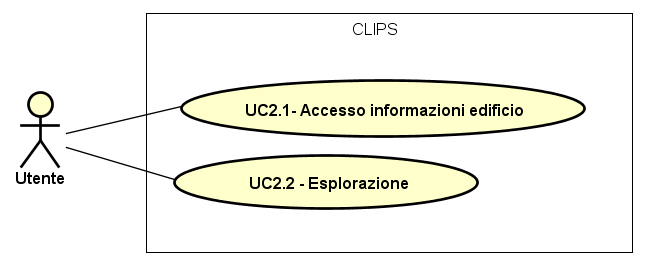
\includegraphics[scale=0.95, width=\textwidth]{img/UC2.png}
            \caption{Caso d'uso UC2: Accesso alle informazioni}\label{fig:UC2} 
        \end{figure}
\begin{itemize}
\item \textbf{Attori}: utente;
\item \textbf{Descrizione}: l'utente deve poter accedere alle informazioni riguardanti le aree vicine alla posizione in cui si trova e le informazioni relative all'edificio in cui si trova; 
      \item \textbf{Precondizione}: l'utente si trova nella sezione dedicata alle informazioni, ha attivato il Bluetooth, si trova all'interno di un edificio mappato e il dispositivo deve rilevare almeno un beacon;

        \item \textbf{Flusso principale degli eventi}:
          \begin{enumerate}
          \item L'utente può accedere alle informazioni dell'edificio (\hyperlink{UC2.1}{UC2.1});
          \item L'utente può accedere alle informazioni delle aree circostanti (\hyperlink{UC2.2}{UC2.2});

      \end{enumerate}
    \item \textbf{Estensioni}:
      \begin{enumerate}
          \item Visualizzazione errore mappa (\hyperlink{UC6}{UC6});

      \end{enumerate}
    \item \textbf{Postcondizione}: il sistema ha presentato all'utente le informazioni richieste.
  \end{itemize}
\hypertarget{UC2.1}{}
\subsection{Caso d'uso UC2.1: Accesso alle informazioni dell'edificio}
\begin{itemize}
\item \textbf{Attori}: utente;
\item \textbf{Descrizione}: l'utente deve poter accedere alle informazioni generali riguardanti l'edificio in cui si trova; 
      \item \textbf{Precondizione}: l'utente si trova nella sezione relativa alle informazioni all'edificio;
    \item \textbf{Postcondizione}: il sistema ha presentato all'utente le informazioni sull'edificio.
  \end{itemize}
\hypertarget{UC2.2}{}
\subsection{Caso d'uso UC2.2: Esplorazione}
\begin{itemize}
\item \textbf{Attori}: utente;
\item \textbf{Descrizione}: l'utente deve poter accedere alle informazioni riguardanti le aree vicine alla sua posizione ed interne all'edificio in cui si trova; 
      \item \textbf{Precondizione}: l'utente si trova nella sezione adibita alle funzionalità di esplorazione;
    \item \textbf{Postcondizione}: il sistema ha presentato all'utente le informazioni riguardanti le aree vicine alla sua posizione attuale.
  \end{itemize}
\hypertarget{UC3}{}
\subsection{Caso d'uso UC3: Gestione dell'applicazione}

        \begin{figure}[!h]
            \centering
            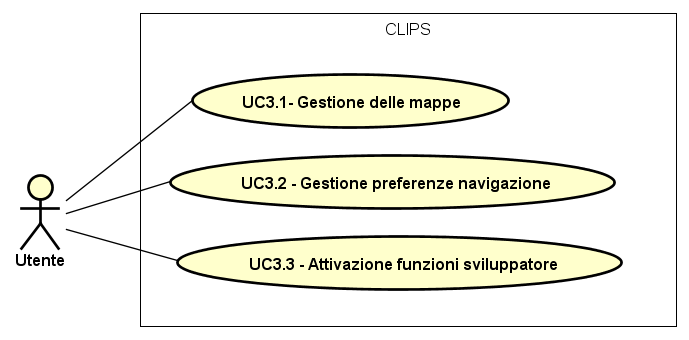
\includegraphics[scale=0.95, width=\textwidth]{img/UC3.png}
            \caption{Caso d'uso UC3: Gestione dell'applicazione}\label{fig:UC3} 
        \end{figure}
\begin{itemize}
\item \textbf{Attori}: utente;
\item \textbf{Descrizione}: l'utente deve poter gestire le mappe utilizzate dall'applicazione e le preferenze relative alle modalità di navigazione. L'utente inoltre deve poter attivare le funzioni avanzate dedicate agli sviluppatori; 
      \item \textbf{Precondizione}: l'utente si trova nella sezione che ospita le opzioni per gestire l'applicazione;

        \item \textbf{Flusso principale degli eventi}:
          \begin{enumerate}
          \item L'utente può accedere alla gestione delle mappe (\hyperlink{UC3.1}{UC3.1});
          \item L'utente può accedere alla gestione delle preferenze di navigazione (\hyperlink{UC3.2}{UC3.2});
          \item L'utente può attivare le funzioni di sviluppatore (\hyperlink{UC3.3}{UC3.3});

      \end{enumerate}
    \item \textbf{Postcondizione}: l'utente ha acceduto alla funzionalità richiesta.
  \end{itemize}
\hypertarget{UC3.1}{}
\subsection{Caso d'uso UC3.1: Gestione mappe}

        \begin{figure}[!h]
            \centering
            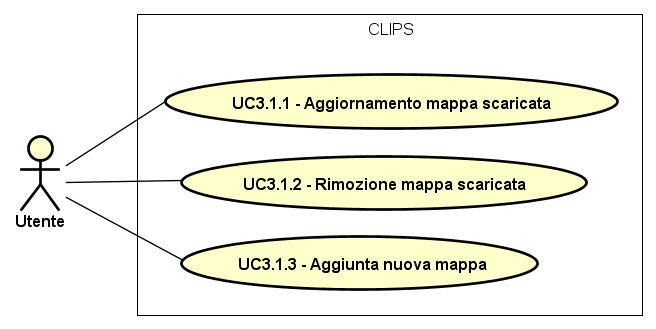
\includegraphics[scale=0.95, width=\textwidth]{img/UC3-1.png}
            \caption{Caso d'uso UC3.1: Gestione mappe}\label{fig:UC3.1} 
        \end{figure}
\begin{itemize}
\item \textbf{Attori}: utente;
\item \textbf{Descrizione}: l'utente deve poter gestire le mappe dei luoghi, fondamentali al funzionamento dell'applicazione; 
      \item \textbf{Precondizione}: l'utente si trova nella sezione adibita alla gestione delle mappe;

        \item \textbf{Flusso principale degli eventi}:
          \begin{enumerate}
          \item L'utente può aggiornare una mappa scaricata in precedenza (\hyperlink{UC3.1.1}{UC3.1.1});
          \item L'utente può rimuovere una mappa scaricata in precedenza (\hyperlink{UC3.1.2}{UC3.1.2});
          \item L'utente può fare il download di una mappa sul proprio dispositivo (\hyperlink{UC3.1.3}{UC3.1.3});

      \end{enumerate}
    \item \textbf{Postcondizione}: il sistema ha erogato la funzionalità richiesta.
  \end{itemize}
\hypertarget{UC3.1.1}{}
\subsection{Caso d'uso UC3.1.1: Aggiornamento mappa scaricata}
\begin{itemize}
\item \textbf{Attori}: utente;
\item \textbf{Descrizione}: l'utente deve poter aggiornare la mappa di un edificio della quale ha effettuato precedentemente il download; 
      \item \textbf{Precondizione}: il dispositivo dell'utente è provvisto di una connessione Internet attiva ed ha abbastanza spazio di archiviazione per la mappa aggiornata;
    \item \textbf{Postcondizione}: la mappa è stata aggiornata.
  \end{itemize}
\hypertarget{UC3.1.2}{}
\subsection{Caso d'uso UC3.1.2: Rimozione mappa scaricata}
\begin{itemize}
\item \textbf{Attori}: utente;
\item \textbf{Descrizione}: l'utente deve poter rimuovere dal dispositivo la mappa di un edificio scaricata in precedenza; 
      \item \textbf{Precondizione}: l'utente ha effettuato precedentemente il download della mappa;
    \item \textbf{Postcondizione}: la mappa è stata rimossa.
  \end{itemize}
\newpage
\hypertarget{UC3.1.3}{}
\subsection{Caso d'uso UC3.1.3: Aggiunta nuova mappa}

        \begin{figure}[!h]
            \centering
            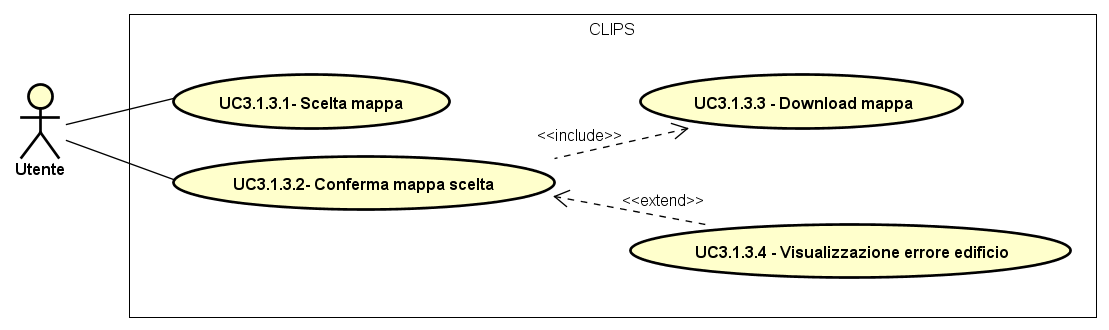
\includegraphics[scale=0.95, width=\textwidth]{img/UC3-1-3.png}
            \caption{Caso d'uso UC3.1.3: Aggiunta nuova mappa}\label{fig:UC3.1.3} 
        \end{figure}
\begin{itemize}
\item \textbf{Attori}: utente;
\item \textbf{Descrizione}: l'utente deve poter effettuare il download della mappa relativa ad uno specifico edificio; 
      \item \textbf{Precondizione}: il dispositivo dell'utente è provvisto di una connessione Internet attiva ed ha abbastanza spazio di archiviazione per la nuova mappa;

        \item \textbf{Flusso principale degli eventi}:
          \begin{enumerate}
          \item L'utente sceglie una mappa tra quelle disponibili (\hyperlink{UC3.1.3.1}{UC3.1.3.1});
          \item L'utente conferma la mappa scelta  (\hyperlink{UC3.1.3.2}{UC3.1.3.2});

      \end{enumerate}
    \item \textbf{Scenari Alternativi}:
      \begin{enumerate}
          \item Nel caso in cui l'utente richieda la mappa di un edificio sconosciuto al sistema viene visualizzato un errore riguardante l'edificio scelto 
 (\hyperlink{UC3.1.3.4}{UC3.1.3.4});

      \end{enumerate}
    \item \textbf{Postcondizione}: la mappa è stata scaricata sul dispositivo dell'utente ed il sistema può utilizzarla.
  \end{itemize}
\hypertarget{UC3.1.3.1}{}
\subsection{Caso d'uso UC3.1.3.1: Scelta mappa}
\begin{itemize}
\item \textbf{Attori}: utente;
\item \textbf{Descrizione}: l'utente deve poter scegliere la mappa relativa ad un certo edificio; 
      \item \textbf{Precondizione}: l'utente è nella sezione dedicata alla scelta delle mappe;
    \item \textbf{Postcondizione}: l'utente ha scelto la mappa dell'edificio desiderato.
  \end{itemize}
\hypertarget{UC3.1.3.2}{}
\subsection{Caso d'uso UC3.1.3.2: Conferma mappa scelta}
\begin{itemize}
\item \textbf{Attori}: utente;
\item \textbf{Descrizione}: l'utente deve poter confermare la mappa scelta per poterne effettuare il download; 
      \item \textbf{Precondizione}: l'utente è nella sezione dedicata alla scelta delle mappe;
    \item \textbf{Estensioni}:
      \begin{enumerate}
          \item Visualizzazione errore edificio (\hyperlink{UC3.1.3.4}{UC3.1.3.4});

      \end{enumerate}
    \item \textbf{Inclusioni}:
      \begin{enumerate}
          \item Download mappa (\hyperlink{UC3.1.3.3}{UC3.1.3.3});

      \end{enumerate}
    \item \textbf{Postcondizione}: l'utente ha scelto la mappa dell'edificio desiderato.
  \end{itemize}
\hypertarget{UC3.1.3.3}{}
\subsection{Caso d'uso UC3.1.3.3: Download mappa}
\begin{itemize}
    \item \textbf{Precondizione}: l'utente ha confermato la mappa da scaricare ed ha abbastanza spazio di archiviazione per la nuova mappa;
    \item \textbf{Postcondizione}: la mappa è presente nel dispositivo.
  \end{itemize}
\hypertarget{UC3.1.3.4}{}
\subsection{Caso d'uso UC3.1.3.4: Visualizzazione errore edificio}
\begin{itemize}
    \item \textbf{Precondizione}: l'utente ha richiesto la mappa di un edificio non riconosciuto dal sistema;
    \item \textbf{Postcondizione}: il sistema visualizza un messaggio di errore riguardante l'impossibilità di scaricare la mappa relativa all'edificio scelto.
  \end{itemize}
\newpage
\hypertarget{UC3.2}{}
\subsection{Caso d'uso UC3.2: Gestione preferenze navigazione}

        \begin{figure}[!h]
            \centering
            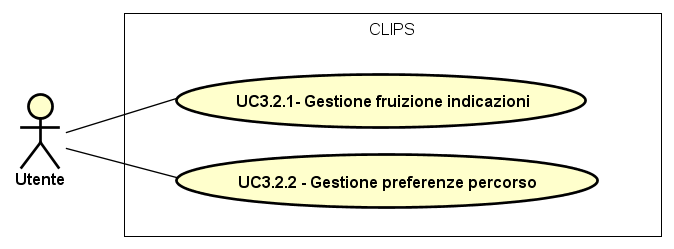
\includegraphics[scale=0.95, width=\textwidth]{img/UC3-2.png}
            \caption{Caso d'uso UC3.2: Gestione preferenze navigazione}\label{fig:UC3.2} 
        \end{figure}
\begin{itemize}
\item \textbf{Attori}: utente;
\item \textbf{Descrizione}: l'utente deve poter gestire le preferenze rispetto a come l'applicazione fornisce indicazioni durante la navigazione e rispetto alle caratteristiche desiderabili che un percorso proposto dovrebbe avere; 
      \item \textbf{Precondizione}: l'utente si trova nella sezione dedicata alla gestione delle preferenze di navigazione;

        \item \textbf{Flusso principale degli eventi}:
          \begin{enumerate}
          \item L'utente può gestire il modo in cui preferisce che le indicazioni gli siano presentate durante la navigazione (\hyperlink{UC3.2.1}{UC3.2.1});
          \item L'utente può gestire le qualità desiderabili che un percorso proposto dovrebbe avere (\hyperlink{UC3.2.2}{UC3.2.2});

      \end{enumerate}
    \item \textbf{Postcondizione}: nel sistema sono state impostate le preferenze dell'utente e verranno applicate a partire dalla prossima volta in cui l'utente avvierà la navigazione.
  \end{itemize}
\hypertarget{UC3.2.1}{}
\subsection{Caso d'uso UC3.2.1: Gestione fruizione indicazioni}

        \begin{figure}[!h]
            \centering
            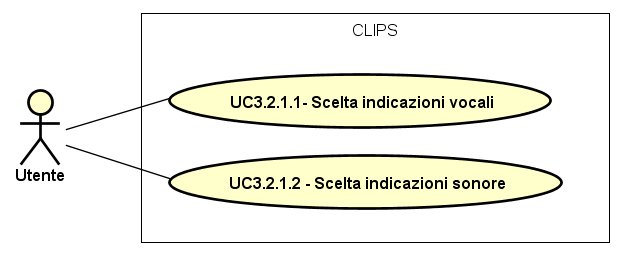
\includegraphics[scale=0.95, width=\textwidth]{img/UC3-2-1.png}
            \caption{Caso d'uso UC3.2.1: Gestione fruizione indicazioni}\label{fig:UC3.2.1} 
        \end{figure}
\begin{itemize}
\item \textbf{Attori}: utente;
\item \textbf{Descrizione}: l'utente deve poter scegliere la modalità con cui preferisce ricevere le indicazioni quando si trova in navigazione; 
      \item \textbf{Precondizione}: l'utente si trova nella sezione dedicata alla gestione della fruizione delle indicazioni;

        \item \textbf{Flusso principale degli eventi}:
          \begin{enumerate}
          \item L'utente può scegliere di ricevere indicazioni vocali (\hyperlink{UC3.2.1.1}{UC3.2.1.1});
          \item L'utente può scegliere di ricevere indicazioni sonore (\hyperlink{UC3.2.1.2}{UC3.2.1.2});

      \end{enumerate}
    \item \textbf{Postcondizione}: nel sistema sono state impostate le preferenze dell'utente rispetto alla fruizione delle indicazioni e verranno applicate a partire dalla prossima volta in cui l'utente avvierà la navigazione.
  \end{itemize}
\hypertarget{UC3.2.1.1}{}
\subsection{Caso d'uso UC3.2.1.1: Scelta indicazioni vocali}
\begin{itemize}
\item \textbf{Attori}: utente;
\item \textbf{Descrizione}: l'utente deve poter scegliere di ricevere indicazioni vocali che lo guidino alla destinazione scelta; 
      \item \textbf{Precondizione}: le indicazioni vocali sono disponibili;
    \item \textbf{Postcondizione}: il sistema fornirà indicazioni vocali partire dalla prossima volta in cui l'utente avvierà la navigazione.
  \end{itemize}
\hypertarget{UC3.2.1.2}{}
\subsection{Caso d'uso UC3.2.1.2: Scelta indicazioni sonore}
\begin{itemize}
\item \textbf{Attori}: utente;
\item \textbf{Descrizione}: l'utente deve poter scegliere di ricevere indicazioni sonore che lo guidino alla destinazione scelta. Questo tipo di indicazioni consiste nell'emissione di un suono monotono continuo la cui frequenza varia con l'allontanamento dell'utente dal percorso previsto. Questo tipo di indicazioni è pensato per agevolare la navigazione di utenti che presentano disabilità visive; 
      \item \textbf{Precondizione}: le indicazioni sonore sono disponibili;
    \item \textbf{Postcondizione}: il sistema fornirà indicazioni sonore partire dalla prossima volta in cui l'utente avvierà la navigazione.
  \end{itemize}
\hypertarget{UC3.2.2}{}
\subsection{Caso d'uso UC3.2.2: Gestione preferenze percorso}

        \begin{figure}[!h]
            \centering
            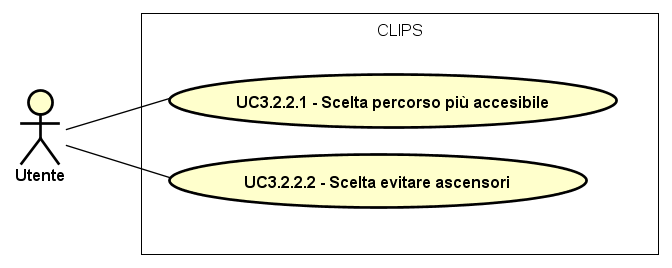
\includegraphics[scale=0.95, width=\textwidth]{img/UC3-2-2.png}
            \caption{Caso d'uso UC3.2.2: Gestione preferenze percorso}\label{fig:UC3.2.2} 
        \end{figure}
\begin{itemize}
\item \textbf{Attori}: utente;
\item \textbf{Descrizione}: l'utente deve poter scegliere le caratteristiche desiderabili che un percorso proposto dovrebbe avere. Queste caratteristiche permettono al sistema di calcolare il percorso più adatto alle necessità dell'utente; 
      \item \textbf{Precondizione}: l'utente si trova nella sezione dedicata alla gestione delle preferenze di percorso;

        \item \textbf{Flusso principale degli eventi}:
          \begin{enumerate}
          \item L'utente può indicare che preferisce il percorso più accessibile (\hyperlink{UC3.2.2.1}{UC3.2.2.1});
          \item L'utente può indicare che preferisce percorsi che non prevedano spazi chiusi e ristretti  (\hyperlink{UC3.2.2.2}{UC3.2.2.2});

      \end{enumerate}
    \item \textbf{Postcondizione}: nel sistema sono state impostate le preferenze dell'utente rispetto ai percorsi e verranno applicate a partire dalla prossima volta in cui l'utente avvierà la navigazione.
  \end{itemize}
\hypertarget{UC3.2.2.1}{}
\subsection{Caso d'uso UC3.2.2.1: Scelta percorso più accessibile}
\begin{itemize}
\item \textbf{Attori}: utente;
\item \textbf{Descrizione}: l'utente deve poter scegliere di ricevere indicazioni per il percorso più accessibile. Il percorso più accessibile è quello che presenta meno barriere architettoniche. Questo tipo di indicazioni è pensato per agevolare la navigazione di utenti che presentano disabilità motorie; 
      \item \textbf{Precondizione}: l'utente si trova nella sezione dedicata alla gestione delle preferenze di percorso;
    \item \textbf{Postcondizione}: il sistema calcolerà il percorso più accessibile a partire dalla prossima volta in cui l'utente avvierà la navigazione.
  \end{itemize}
\hypertarget{UC3.2.2.2}{}
\subsection{Caso d'uso UC3.2.2.2: Scelta evitare ascensori}
\begin{itemize}
\item \textbf{Attori}: utente;
\item \textbf{Descrizione}: l'utente deve poter scegliere di ricevere indicazioni per il percorso che presenta il minor numero di ascensori. Questo tipo di indicazioni è pensato per agevolare la navigazione di utenti claustrofobici; 
      \item \textbf{Precondizione}: l'utente si trova nella sezione dedicata alla gestione delle preferenze di percorso;
    \item \textbf{Postcondizione}: il sistema calcolerà il percorso col minor numero di ascensori a partire dalla prossima volta in cui l'utente avvierà la navigazione.
  \end{itemize}
\hypertarget{UC3.3}{}
\subsection{Caso d'uso UC3.3: Attivazione funzionalità sviluppatore}

        \begin{figure}[!h]
            \centering
            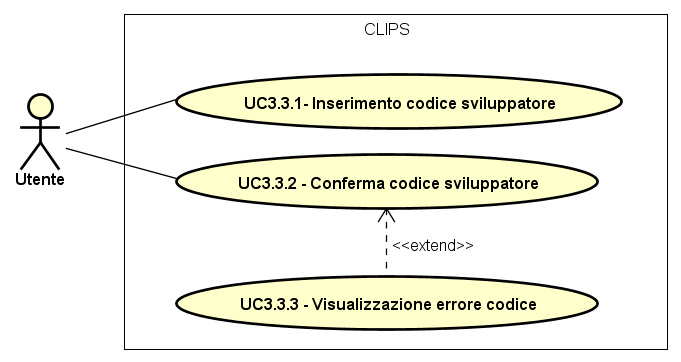
\includegraphics[scale=0.95, width=\textwidth]{img/UC3-3.png}
            \caption{Caso d'uso UC3.3: Attivazione funzionalità sviluppatore}\label{fig:UC3.3} 
        \end{figure}
\begin{itemize}
\item \textbf{Attori}: utente;
\item \textbf{Descrizione}: un utente, se è in possesso di un codice sviluppatore valido, deve poter attivare le funzionalità avanzate dedicate agli sviluppatori offerte dall'applicazione; 
      \item \textbf{Precondizione}: l'utente si trova nella sezione dedicata all'attivazione delle funzionalità sviluppatore e l'utente non è già sviluppatore;

        \item \textbf{Flusso principale degli eventi}:
          \begin{enumerate}
          \item L'utente inserisce il codice sviluppatore (\hyperlink{UC3.3.1}{UC3.3.1});
          \item L'utente conferma il codice inserito (\hyperlink{UC3.3.2}{UC3.3.2});

      \end{enumerate}
    \item \textbf{Scenari Alternativi}:
      \begin{enumerate}
          \item Nel caso in cui l'utente inserisca un codice sviluppatore non valido viene visualizzato un errore riguardante il codice inserito (\hyperlink{UC3.3.3}{UC3.3.3});

      \end{enumerate}
    \item \textbf{Postcondizione}: il sistema rende disponibili le funzionalità sviluppatore.
  \end{itemize}
\hypertarget{UC3.3.1}{}
\subsection{Caso d'uso UC3.3.1: Inserimento codice sviluppatore}
\begin{itemize}
\item \textbf{Attori}: utente;
\item \textbf{Descrizione}: l'utente deve poter inserire un codice per poter accedere alle funzionalità sviluppatore; 
      \item \textbf{Precondizione}: l'utente non ha mai inserito un codice valido prima;
    \item \textbf{Postcondizione}: il codice sviluppatore è stato inserito.
  \end{itemize}
\hypertarget{UC3.3.2}{}
\subsection{Caso d'uso UC3.3.2: Conferma codice}
\begin{itemize}
\item \textbf{Attori}: utente;
\item \textbf{Descrizione}: l'utente deve poter confermare il codice sviluppatore inserito; 
      \item \textbf{Precondizione}: l'utente ha inserito un codice nell'apposita sezione;
    \item \textbf{Estensioni}:
      \begin{enumerate}
          \item Visualizzazione errore codice (\hyperlink{UC3.3.3}{UC3.3.3});

      \end{enumerate}
    \item \textbf{Postcondizione}: il sistema permette l'accesso alle funzionalità sviluppatore.
  \end{itemize}
\hypertarget{UC3.3.3}{}
\subsection{Caso d'uso UC3.3.3: Visualizzazione errore codice}
\begin{itemize}
    \item \textbf{Precondizione}: l'utente ha inserito un codice sviluppatore non valido;
    \item \textbf{Postcondizione}: il sistema non permette l'accesso alle funzionalità sviluppatore.
  \end{itemize}
\hypertarget{UC4}{}
\subsection{Caso d'uso UC4: Accesso alla guida}
\begin{itemize}
\item \textbf{Attori}: utente;
\item \textbf{Descrizione}: l'utente deve poter accedere ad una guida che illustri l'utilizzo del prototipo; 
      \item \textbf{Precondizione}: il sistema mette a disposizione una sezione che ospita la guida;
    \item \textbf{Postcondizione}: il sistema ha visualizzato la guida.
  \end{itemize}
  \newpage
\hypertarget{UC5}{}
\subsection{Caso d'uso UC5: Accesso funzionalità sviluppatore}

        \begin{figure}[!h]
            \centering
            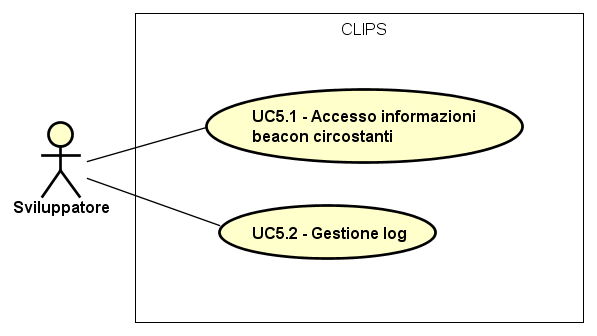
\includegraphics[scale=0.95, width=\textwidth]{img/UC5.png}
            \caption{Caso d'uso UC5: Accesso funzionalità sviluppatore}\label{fig:UC5} 
        \end{figure}
\begin{itemize}
\item \textbf{Attori}: sviluppatore;
\item \textbf{Descrizione}: lo sviluppatore deve poter accedere alle funzionalità avanzate messe a disposizione dall'applicazione. Tali funzionalità sono rivolte a testare e migliorare l'applicazione ed il sistema con il quale interagisce; 
      \item \textbf{Precondizione}: lo sviluppatore si trova nella sezione dedicata alle funzionalità avanzate dell'applicazione;

        \item \textbf{Flusso principale degli eventi}:
          \begin{enumerate}
          \item Lo sviluppatore può accedere alle informazioni relative ai beacon circostanti (\hyperlink{UC5.1}{UC5.1});
          \item Lo sviluppatore può gestire i log (\hyperlink{UC5.2}{UC5.2});

      \end{enumerate}
    \item \textbf{Postcondizione}: lo sviluppatore ha usufruito delle funzionalità avanzate.
  \end{itemize}
\hypertarget{UC5.1}{}
\subsection{Caso d'uso UC5.1: Accesso informazioni beacon circostanti}
\begin{itemize}
\item \textbf{Attori}: sviluppatore;
\item \textbf{Descrizione}: lo sviluppatore deve poter accedere alle informazioni relative ai beacon presenti nelle vicinanze. Tali informazioni riguardano: UUID, Major, Minor, livello di potenza del segnale, livello batteria, distanza approssimativa, formato del beacon, area coperta dal beacon; 
      \item \textbf{Precondizione}: lo sviluppatore si trova nella sezione dedicata alle informazioni sui beacon circostanti ed ha il Bluetooth attivato;
    \item \textbf{Postcondizione}: lo sviluppatore ha usufruito delle informazioni sui beacon circostanti.
  \end{itemize}
\hypertarget{UC5.2}{}
\subsection{Caso d'uso UC5.2: Gestione log}

        \begin{figure}[!h]
            \centering
            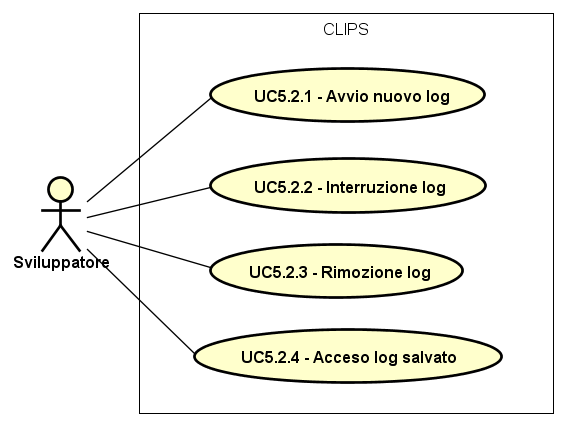
\includegraphics[scale=0.95, width=\textwidth]{img/UC5-2.png}
            \caption{Caso d'uso UC5.2: Gestione log}\label{fig:UC5.2} 
        \end{figure}
\begin{itemize}
\item \textbf{Attori}: sviluppatore;
\item \textbf{Descrizione}: lo sviluppatore deve poter accedere alla gestione del log. Il log contiene tutte le informazioni indicate in \hyperlink{UC5.1}{UC5.1} e relative ai beacon rilevati durante la registrazione del log. Lo sviluppatore può decidere quando avviare e interrompere la registrazione del log; 
      \item \textbf{Precondizione}: lo sviluppatore si trova nella sezione dedicata alla gestione del log;

        \item \textbf{Flusso principale degli eventi}:
          \begin{enumerate}
          \item Lo sviluppatore può avviare un nuovo log (\hyperlink{UC5.2.1}{UC5.2.1});
          \item Lo sviluppatore può interrompere un log in corso (\hyperlink{UC5.2.2}{UC5.2.2});
          \item Lo sviluppatore può rimuovere un log salvato (\hyperlink{UC5.2.3}{UC5.2.3});
          \item Lo sviluppatore può accedere ad un log salvato (\hyperlink{UC5.2.4}{UC5.2.4});

      \end{enumerate}
    \item \textbf{Postcondizione}: lo sviluppatore ha usufruito della gestione del log.
  \end{itemize}
\hypertarget{UC5.2.1}{}
\subsection{Caso d'uso UC5.2.1: Avvio nuovo log}
\begin{itemize}
\item \textbf{Attori}: sviluppatore;
\item \textbf{Descrizione}: lo sviluppatore deve poter avviare un nuovo log; 
      \item \textbf{Precondizione}: lo sviluppatore si trova nella sezione dedicata alla gestione dei log;
    \item \textbf{Postcondizione}: il sistema ha creato ed avviato un nuovo log.
  \end{itemize}
\hypertarget{UC5.2.2}{}
\subsection{Caso d'uso UC5.2.2: Interruzione log}
\begin{itemize}
\item \textbf{Attori}: sviluppatore;
\item \textbf{Descrizione}: lo sviluppatore deve poter interrompere un log in corso; 
      \item \textbf{Precondizione}: lo sviluppatore si trova nella sezione dedicata alla gestione dei log;
    \item \textbf{Postcondizione}: il sistema ha salvato il log.
  \end{itemize}
\hypertarget{UC5.2.3}{}
\subsection{Caso d'uso UC5.2.3: Rimozione log}
\begin{itemize}
\item \textbf{Attori}: sviluppatore;
\item \textbf{Descrizione}: lo sviluppatore deve poter rimuovere un log salvato; 
      \item \textbf{Precondizione}: è presente almeno un log;
    \item \textbf{Postcondizione}: il sistema ha cancellato il log da rimuovere.
  \end{itemize}
\hypertarget{UC5.2.4}{}
\subsection{Caso d'uso UC5.2.4: Accesso log salvato}
\begin{itemize}
\item \textbf{Attori}: sviluppatore;
\item \textbf{Descrizione}: lo sviluppatore deve poter accedere ad un log salvato; 
      \item \textbf{Precondizione}: è presente almeno un log;
    \item \textbf{Postcondizione}: il sistema ha fornito le informazioni contenute nel log.
  \end{itemize}
\hypertarget{UC6}{}
\subsection{Caso d'uso UC6: Visualizzazione errore mappa}
\begin{itemize} 
    \item \textbf{Precondizione}: l'utente non possiede la mappa dell'edificio in cui sta utilizzando l'applicazione oppure la mappa non è aggiornata;
    \item \textbf{Postcondizione}: il sistema ha visualizzato un messaggio di errore.
  \end{itemize}
 \end{document}